\begin{figure}[h!]
    \centering
    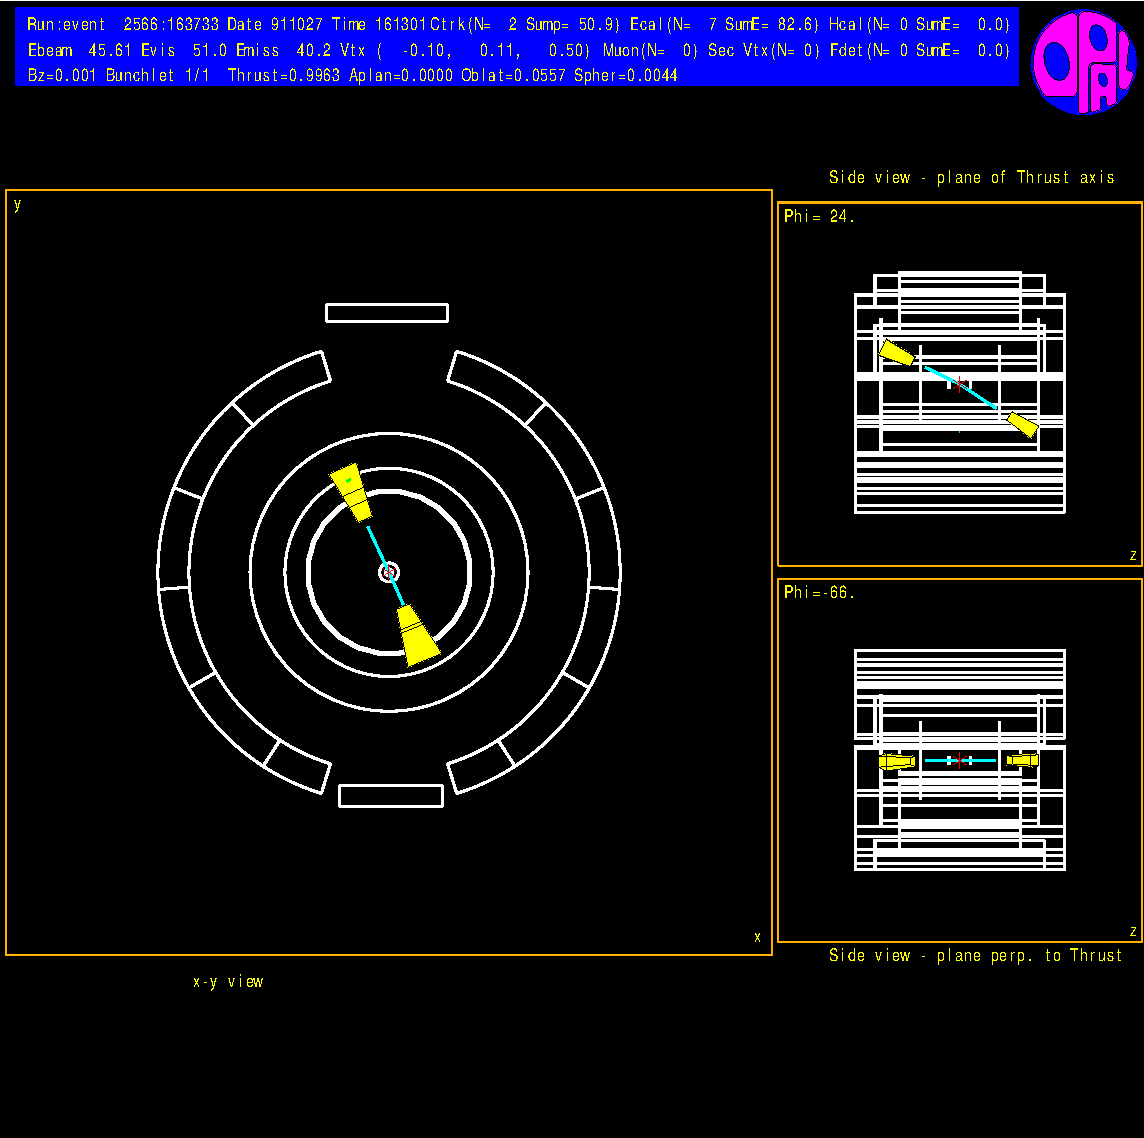
\includegraphics[width = 8cm]{part1ee.pdf}
    \caption{Event display of $e^-e^+$-channel sample}
    \label{fig:part1ee}
\end{figure}

\begin{figure}[h!]
    \centering
    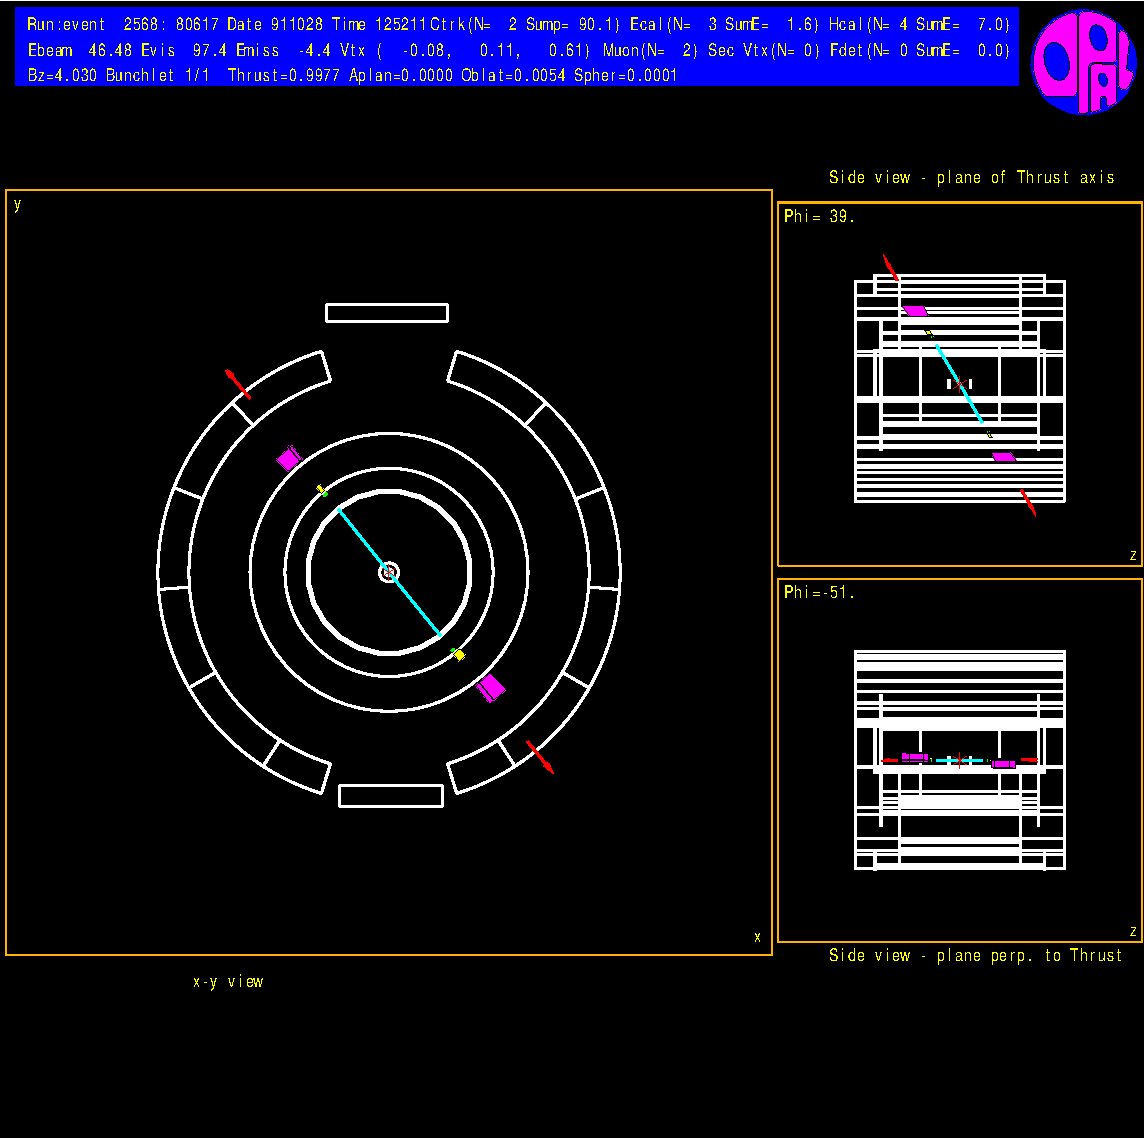
\includegraphics[width = 8cm]{part1mm.pdf}
    \caption{Event display of $\mu^-\mu^+$-channel sample}
    \label{fig:part1mm}
\end{figure}

\begin{figure}[h!]
    \centering
    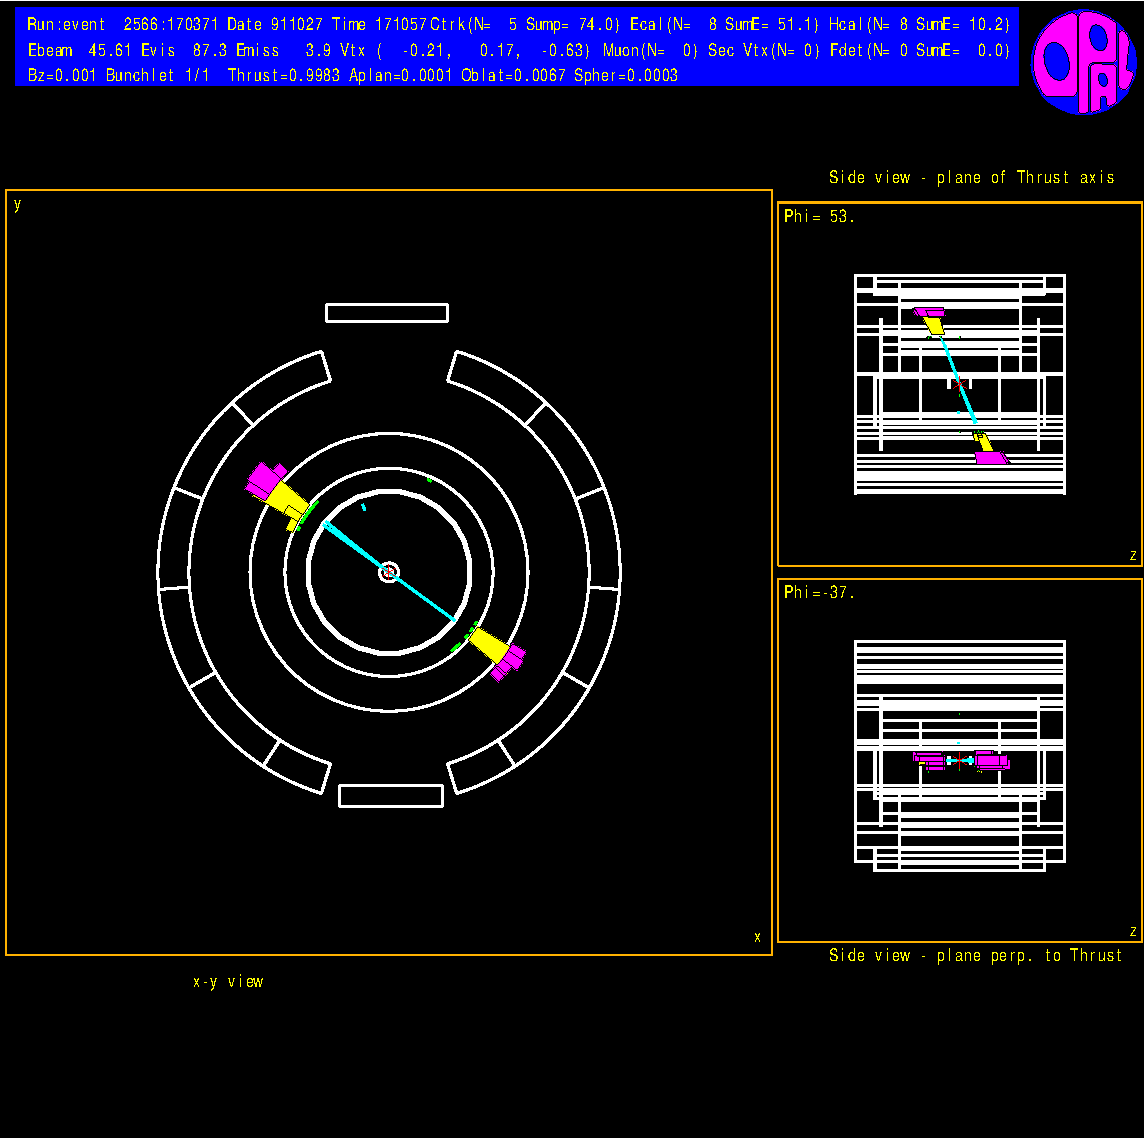
\includegraphics[width = 8cm]{part1tt.pdf}
    \caption{Event display of $\tau^-\tau^+$-channel sample}
    \label{fig:part1tt}
\end{figure}

\begin{figure}[h!]
    \centering
    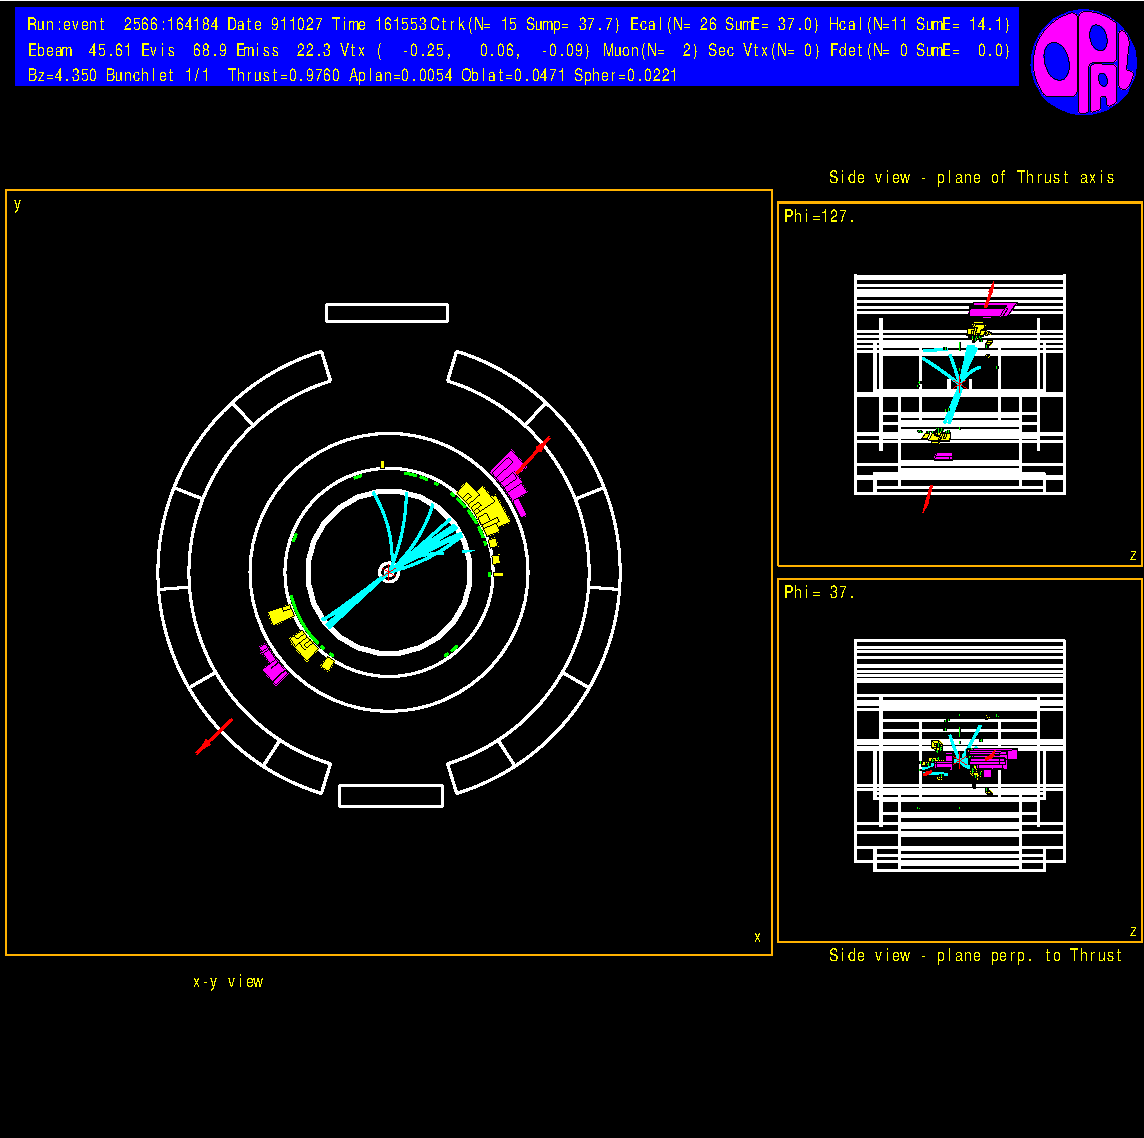
\includegraphics[width = 8cm]{part1qq.pdf}
    \caption{Event display of $q\bar{q}$-channel sample}
    \label{fig:part1qq}
\end{figure}

\begin{figure}[h!]
    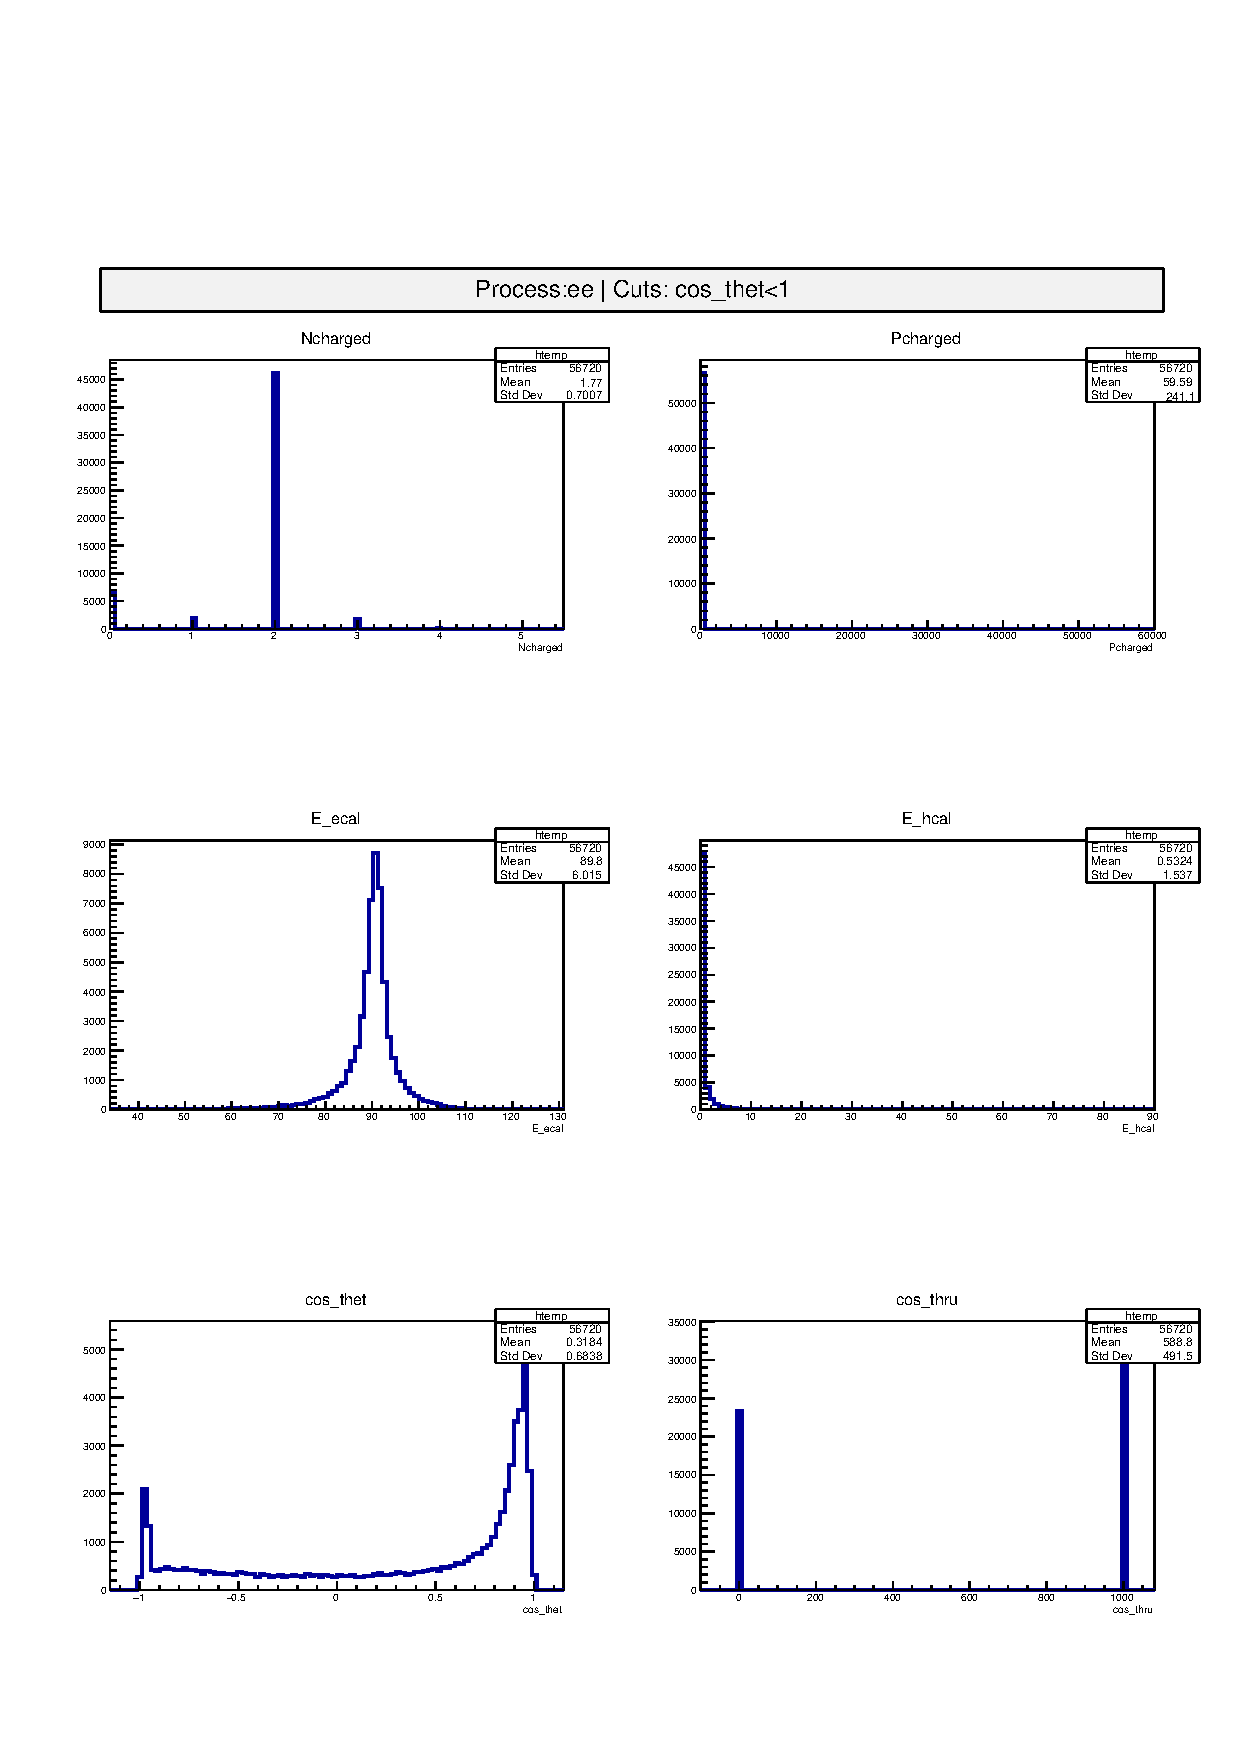
\includegraphics[scale = 0.8]{globalcut_ee.pdf}
    \caption{Global cuts applied to $e^-e^+$ MC}
    \label{fig:global-ee}
\end{figure}

\begin{figure}[h!]
    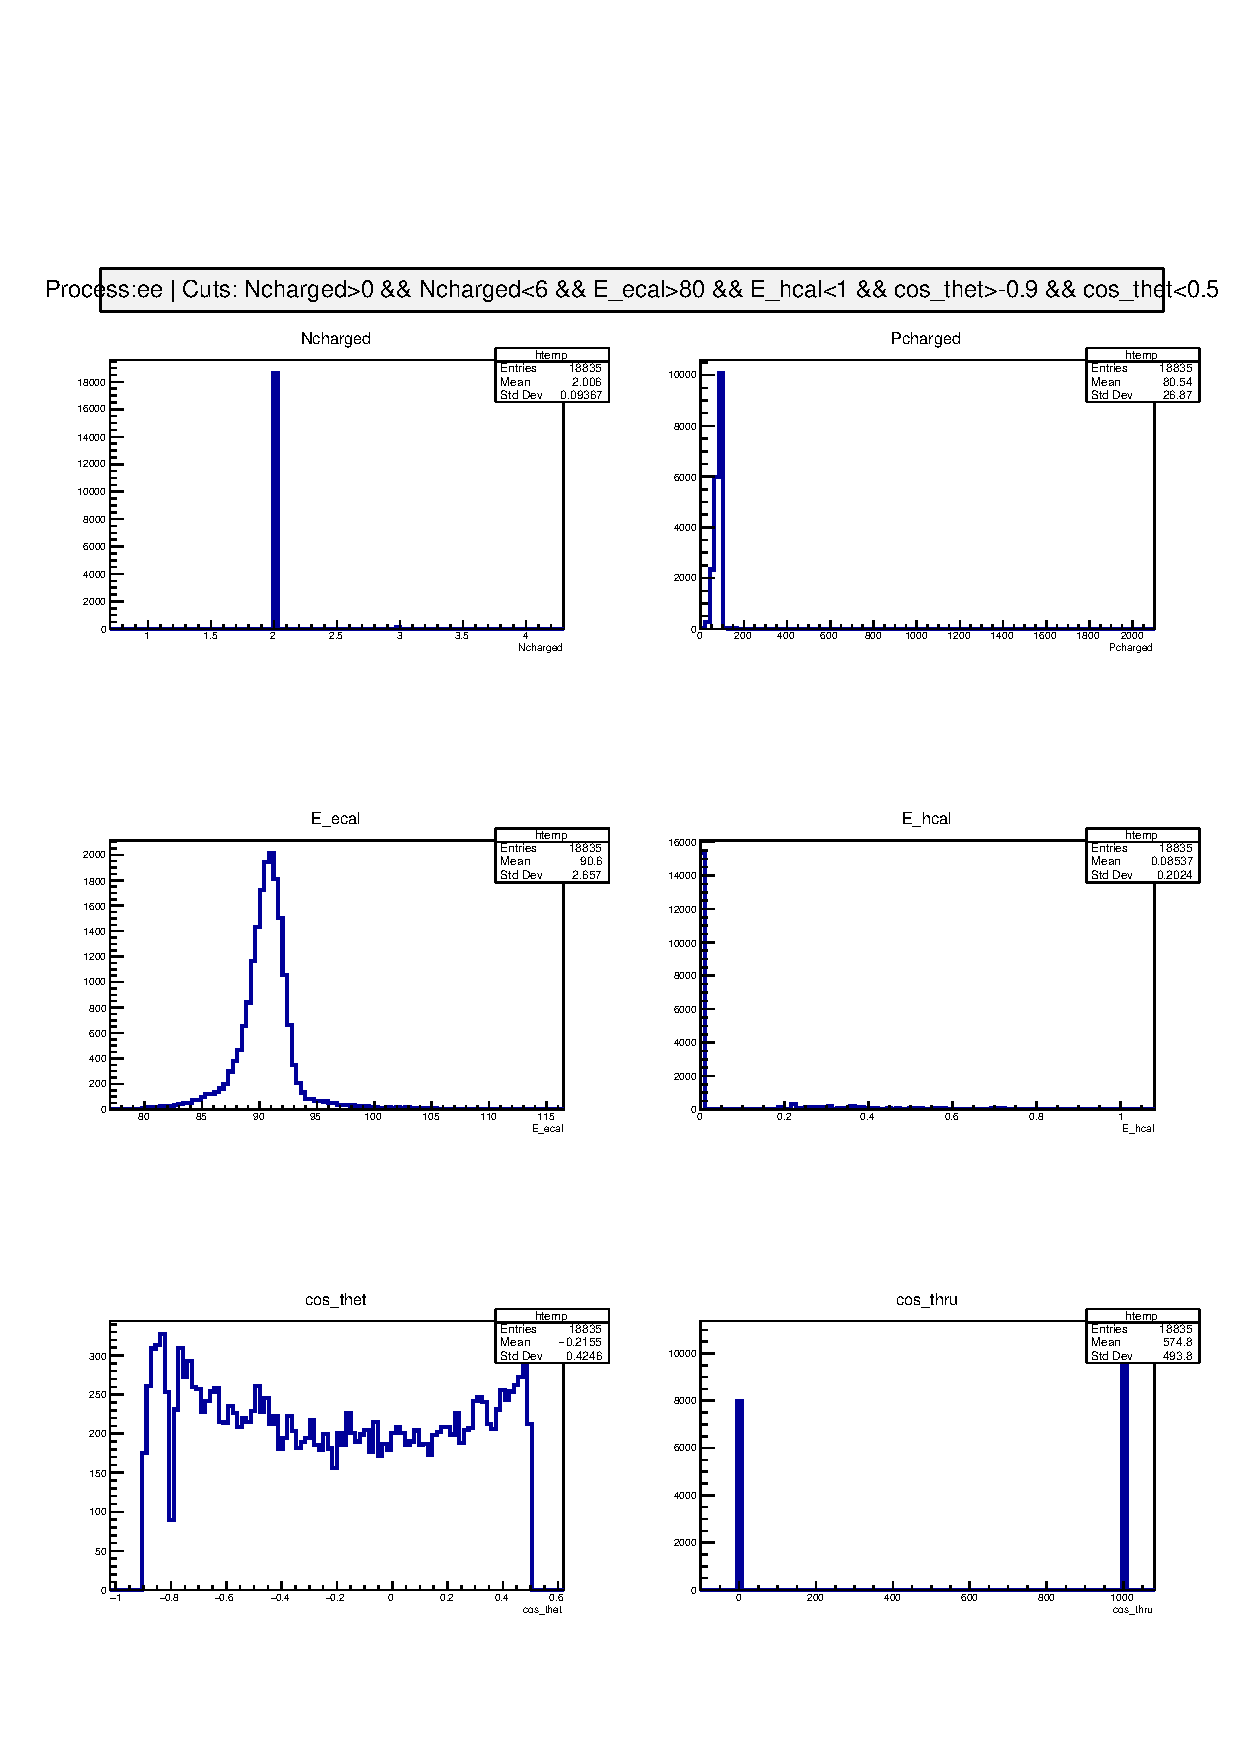
\includegraphics[scale = 0.8]{ee_cut_on_ee.pdf}
    \caption{$e^-e^+$ cuts applied to $e^-e^+$ MC}
    \label{fig:eecutee}
\end{figure}

\begin{figure}[h!]
    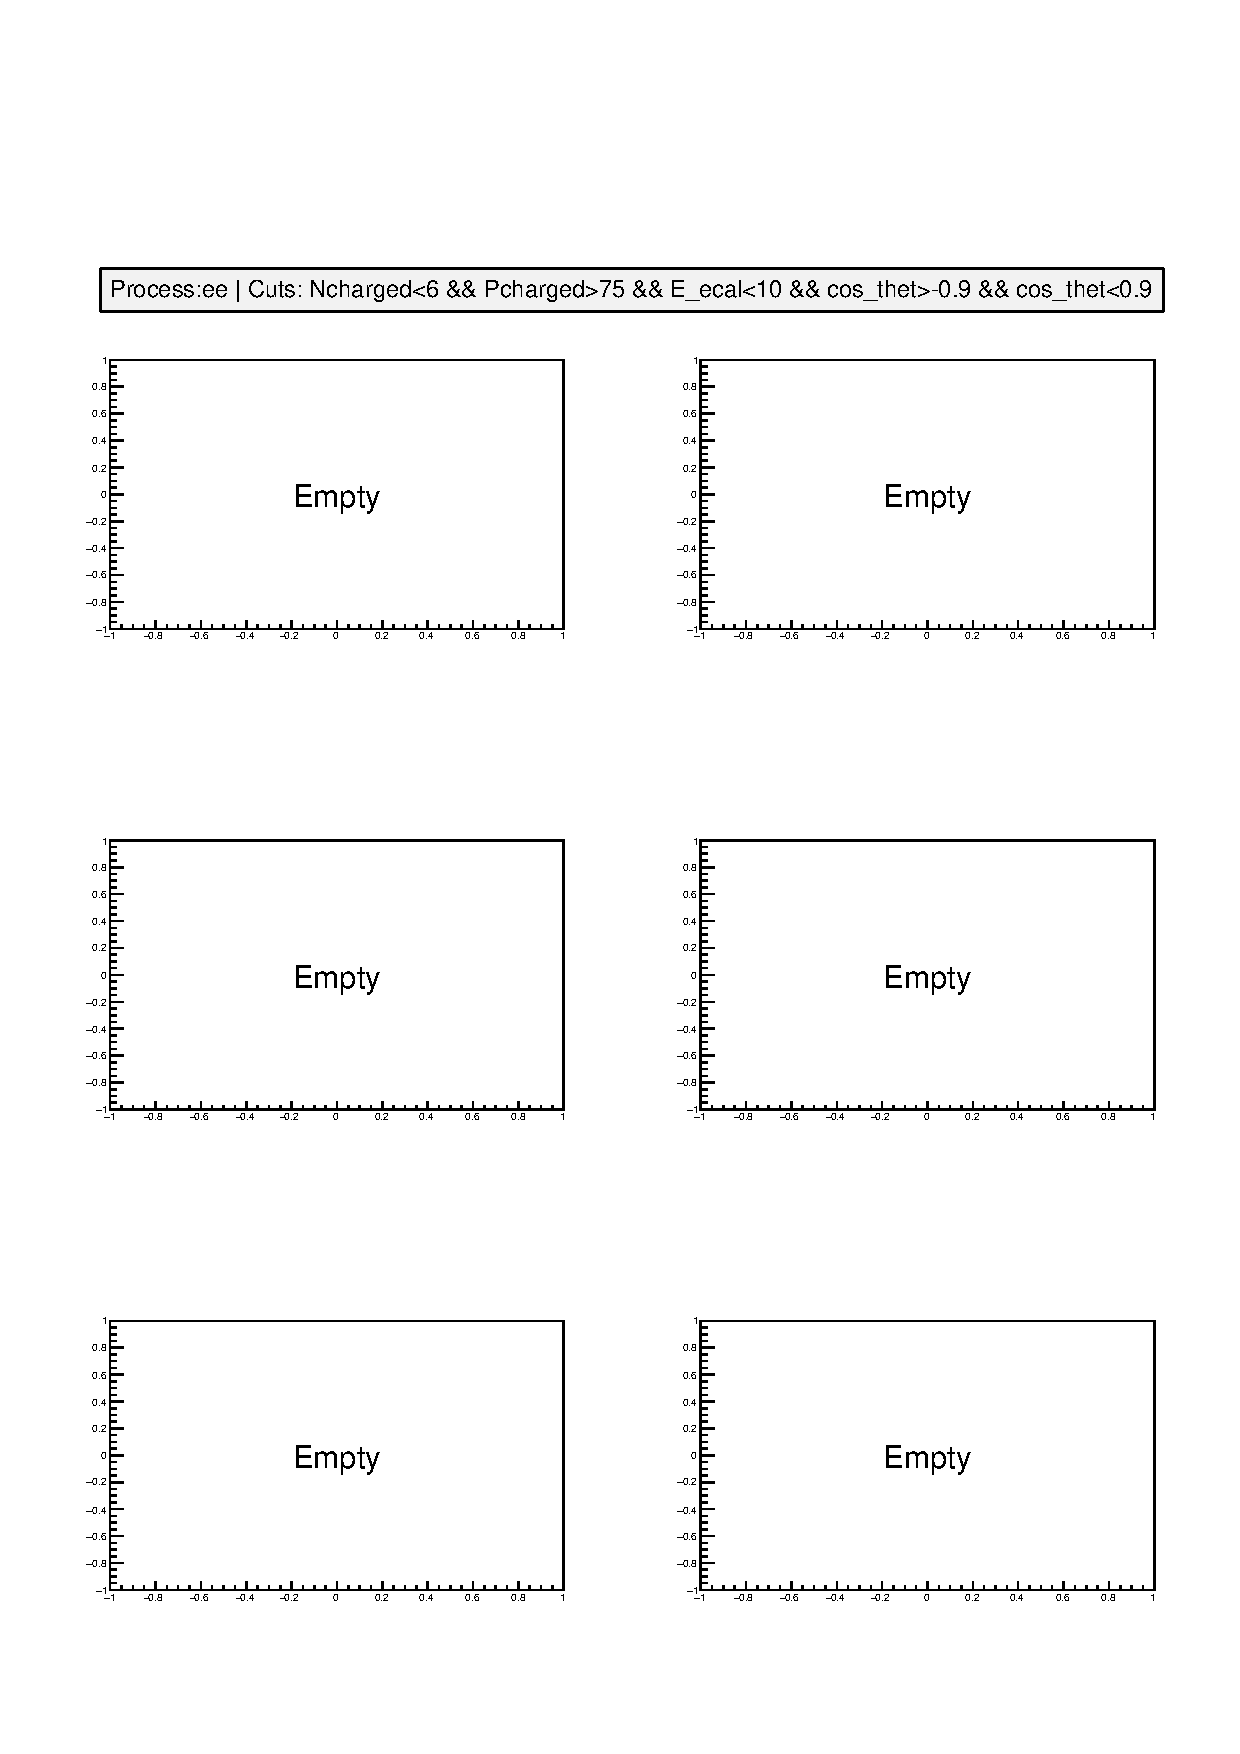
\includegraphics[scale = 0.8]{mm_cut_on_ee.pdf}
    \caption{$\mu^-\mu^+$ cuts applied to $e^-e^+$ MC}
    \label{fig:mmcutee}
\end{figure}

\begin{figure}[h!]
    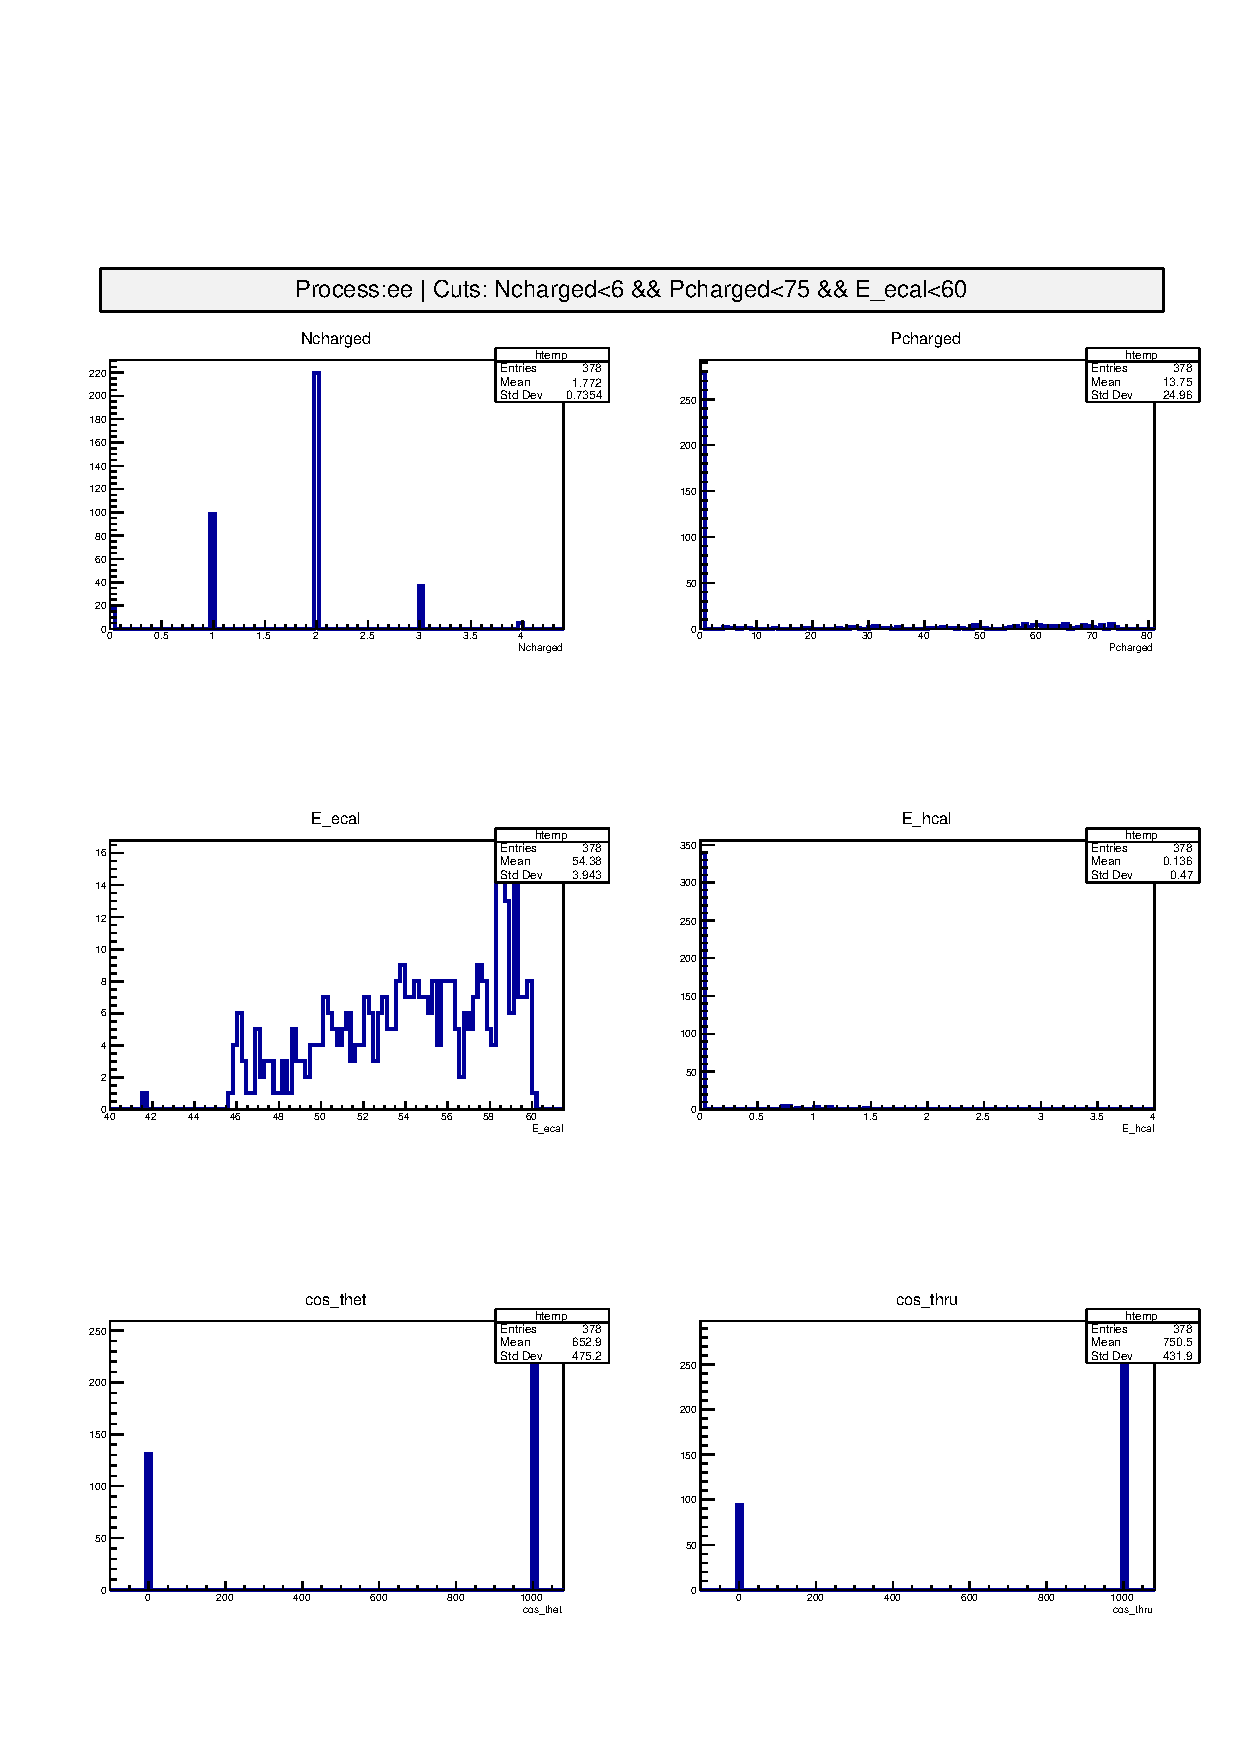
\includegraphics[scale = 0.8]{tt_cut_on_ee.pdf}
    \caption{$\tau^-\tau^+$ cuts applied to $e^-e^+$ MC}
    \label{fig:ttcutee}
\end{figure}

\begin{figure}[h!]
    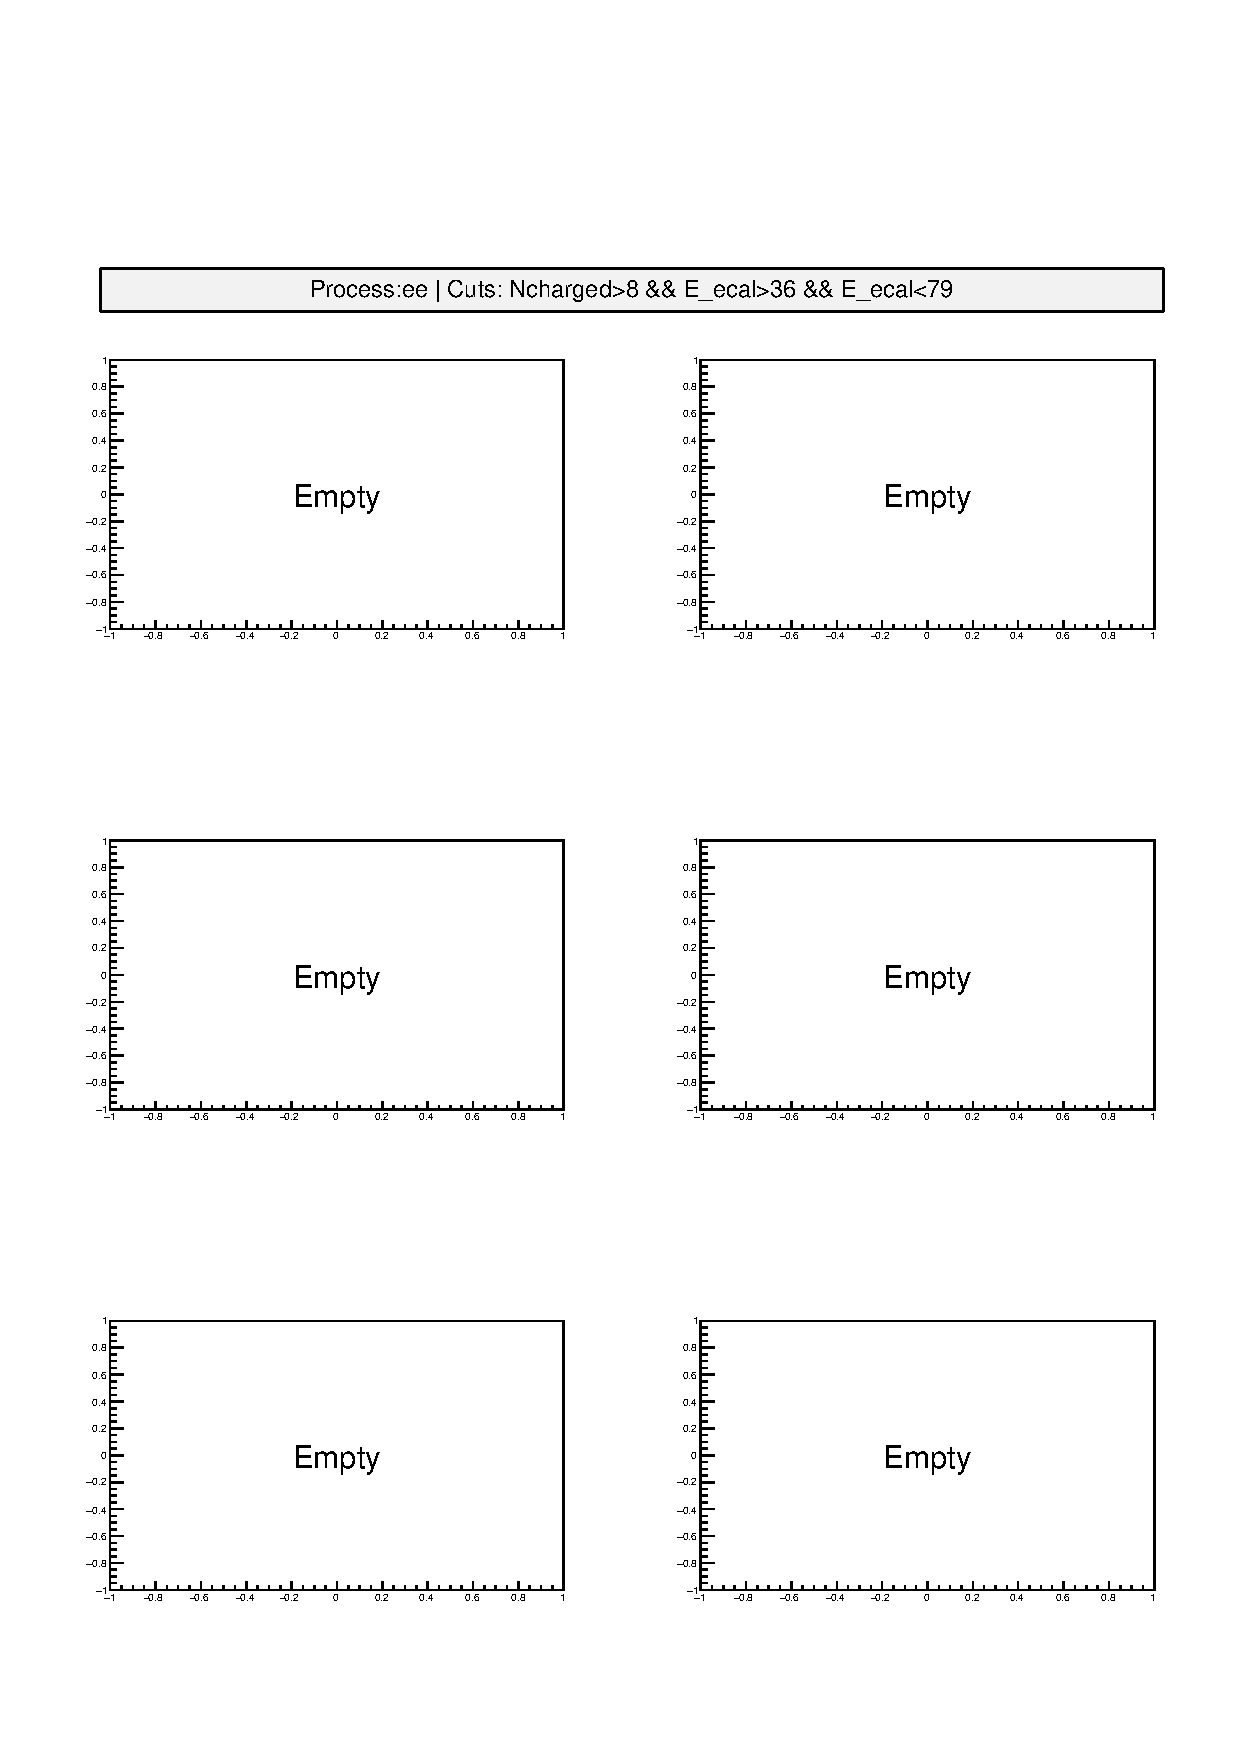
\includegraphics[scale = 0.8]{qq_cut_on_ee.pdf}
    \caption{$q\bar{q}$ cuts applied to $e^-e^+$ MC}
    \label{fig:qqcutee}
\end{figure}